\documentclass{article} 
\usepackage[left=0.75in,top=0.6in,right=0.75in,bottom=0.6in]{geometry} % Document margins
\usepackage{tabularx}
\usepackage{fancyvrb}
%\usepackage[hidelinks]{hyperref}
\usepackage{graphicx}
\usepackage{float}
\usepackage{fancyhdr}
\usepackage{geometry}
\usepackage{lastpage}
\usepackage{tabu}
\usepackage{hyperref}



\geometry{
  top=1in,            % <-- you want to adjust this
  inner=0.5in,
  outer=0.5in,
  bottom=1in,
  headheight=5ex,       % <-- and this
  headsep=4ex,          % <-- and this
}

\pagestyle{fancy}
\fancyhf{}
\rhead{\Large\textit{Old Dominion University}}
\lhead{\Large\textit{ECE 432: Assignment 10}}
\cfoot{Page \thepage \hspace{1pt} of \pageref{LastPage}}
\renewcommand{\footrulewidth}{1pt}

\begin{document}

%----------------------------------------------------------------------------------------
%		 TITLE PAGE
%----------------------------------------------------------------------------------------

\begin{titlepage}

\vspace*{45 pt}
\begin{center}
\Huge{\bf CS 432/532:  Web Science}\\
\huge{Spring 2017\\}

\vspace{60 pt}
\Huge\underline {Assignment 10}\\

\vspace{10 pt}
\Huge{Michael Micros}\\\

{\Large \bf {Instructor: Michael L. Nelson}}\\

\vspace{230 pt}
{\huge \bf {Old Dominon University}}\\
{\huge \bf {Norfolk, Virginia}}\\

\vspace{10 pt}
\today

\end{center}
\end{titlepage}




%----------------------------------------------------------------------------------------
%		PROBLEM 1
%----------------------------------------------------------------------------------------

\section*{{\underline{\huge {Problem 1:}} Computing kNN for Dr. Nelson's blogs}}
 Having substituted the euclidean distance with the cosine, the Knn function provided in the ``Programming Collective Intelligence" textbook was used on the blogdata collected in Assignment 8. The blog data are located in ``blogdata.txt". 

\begin{figure}[H]
 \centering
 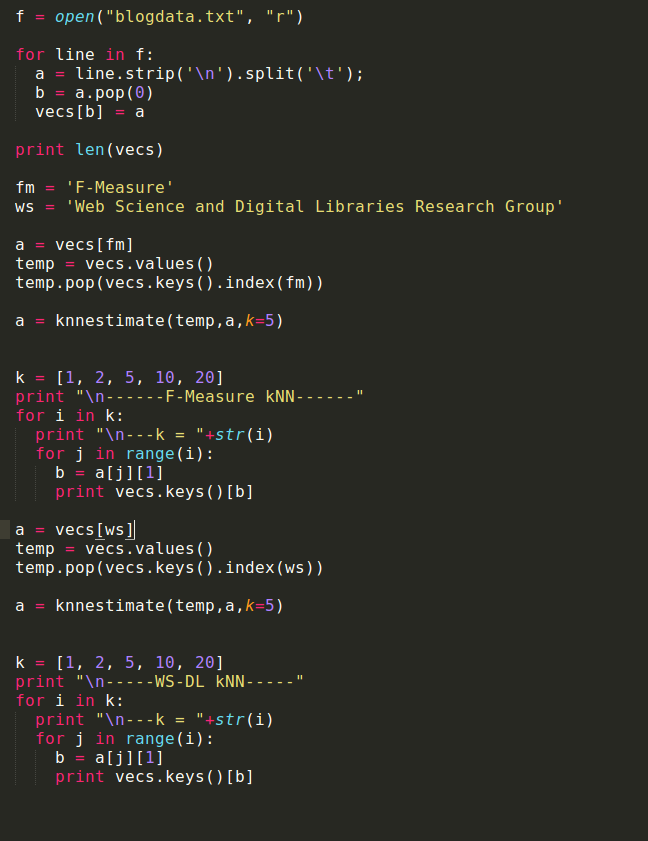
\includegraphics[width=14 cm]{code.png}
  \caption{Code for calculating kNN for F-Measure and WS-DL.}
\end{figure}

\begin{figure}[H]
 \centering
 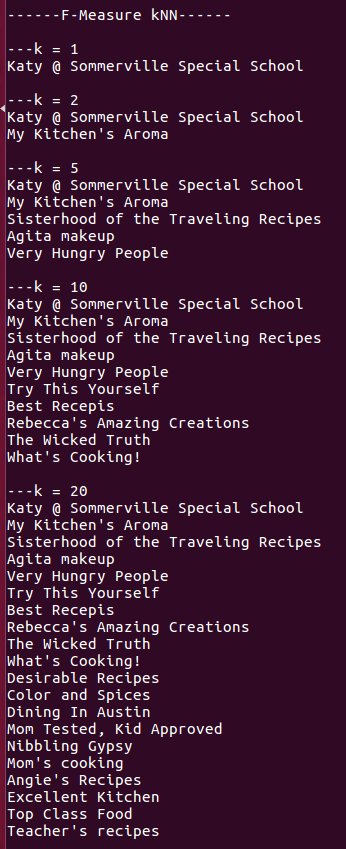
\includegraphics[width=8 cm]{fmes.png}
  \caption{kNN results for http://f-measure.blogspot.com/.}
\end{figure}

\begin{figure}[H]
 \centering
 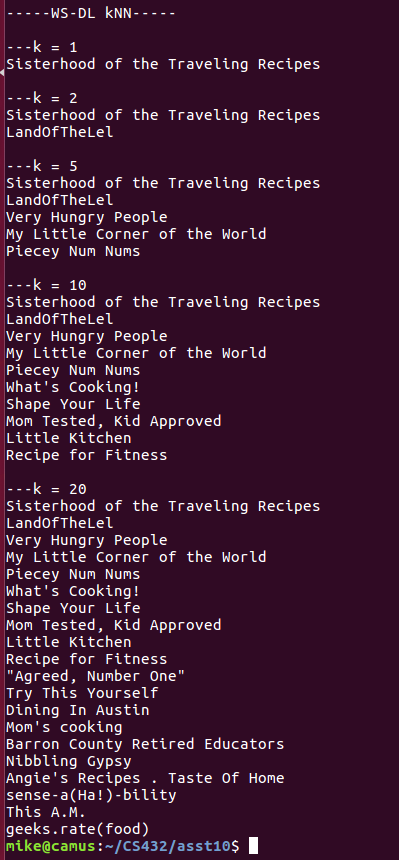
\includegraphics[width=8 cm]{ws.png}
  \caption{kNN results for http://ws-dl.blogspot.com/.}
\end{figure}

%----------------------------------------------------------------------------------------
%		PROBLEM 2
%----------------------------------------------------------------------------------------

\section*{{\underline{\huge {Problem 2:}} LIBSVM  }}




%----------------------------------------------------------------------------------------
\end{document}
